\section{Results}
\label{Benchmarking:Results}

We provide now the results of the execution of the privacy filters, with the configuration specified in the previous section. For each filter, we present summary tables with the disclosure risk and information loss estimates for each parameterization, as well as plots showing the evolution of both measurements against the number of instances processed.

\subsection{Noise addition}
\label{Benchmarking:Results:Noise}

All the considered parameterizations for the \texttt{NoiseAdditionFilter} are reflected on~\tref{table:results-rbf-noise-addition} and~\tref{table:results-wave-noise-addition}. The evolution of disclosure risk against the number of instances processed is shown in~\fref{fig:results-dr-na} and information loss is shown in~\fref{fig:results-il-log-na}.

\begin{minipage}[t]{0.5\textwidth}
	\begin{flushleft}
	\begin{table}[H]
		\centering
		\begin{tabular}{@{}rrrr@{}}
			\toprule
			$a$ & $c$ & \multicolumn{1}{c}{DR} & \multicolumn{1}{c}{IL} \\ \midrule
			0.1 & 0.0 & 0.956	& 1123.97 \\
			0.25 & 0.0 & 0.889 & 7024.83 \\
			0.5 & 0.0 & 0.774	& 28099.33 \\
			0.75 & 0.0 & 0.596 & 63223.50 \\
			1.0 & 0.0 & 0.430 & 112397.34 \\ \bottomrule
		\end{tabular}
		\caption[Noise addition DR \& IL estimations (\texttt{RandomRBFGenerator}).]{Noise addition IL \& DR estimations for all considered parameterizations with the \texttt{RandomRBFGenerator}.}
		\label{table:results-rbf-noise-addition}
	\end{table}
	\end{flushleft}
\end{minipage}
\begin{minipage}[t]{0.5\textwidth}
	\begin{flushright}
	\begin{table}[H]
		\centering
		\begin{tabular}{@{}rrrr@{}}
			\toprule
			$a$ & $c$ & \multicolumn{1}{c}{DR} & \multicolumn{1}{c}{IL} \\ \midrule
			0.1  & 0.0 & 1.000 & 50741.41   \\
			0.25 & 0.0 & 1.000 & 317133.83  \\
			0.5  & 0.0 & 0.996 & 1268535.34 \\
			0.75 & 0.0 & 0.919 & 2854204.53 \\
			1.0  & 0.0 & 0.742 & 5074141.39 \\ \bottomrule
		\end{tabular}
		\caption[Noise addition DR \& IL estimations (\texttt{WaveformGenerator}).]{Noise addition IL \& DR estimations for all considered parameterizations with the \texttt{WaveformGenerator}.}
		\label{table:results-wave-noise-addition}
	\end{table}
	\end{flushright}
\end{minipage}

As was anticipated in the theoretical introduction chapter, the \texttt{NoiseAdditionFilter} is not able to protect data as much as other methods do. The results of its application on the \texttt{RandomRBFGenerator} data prove to be much better than on the \texttt{WaveformGenerator}, on which has almost no effect at all. Even the high amount of noise introduced, it is not really protecting data against disclosure --- although the $a$ control parameter of the filter is set to its maximum value ($a = 1$), the disclosure risk is quite high.

The effect of the noise scaling factor controlled by the $a$ parameter can cleary be seen on~\fref{fig:results-il-log-na}: the higher the value of the parameter, the higher the information loss. Another important thing to notice is that the amount of noise added for each instance remains constant, this is, the increment in the total information loss measure grows linearly.

\begin{figure}[h]
	\centering
	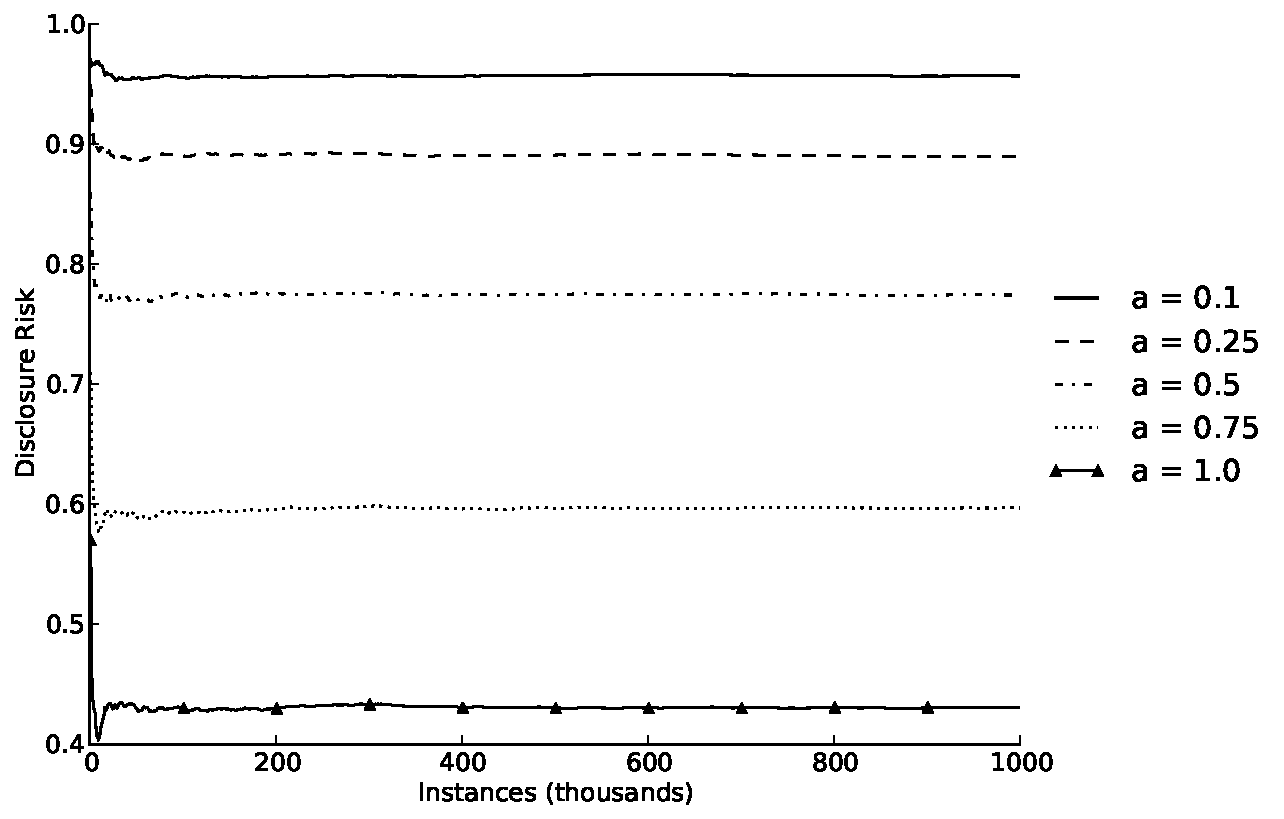
\includegraphics[width=0.9\linewidth]{figures/dr_na-random.pdf}
	\caption[Noise addition DR evaluation ($c = 0$).]{\texttt{NoiseAdditionFilter} DR evaluation using the \texttt{RandomRBFGenerator} with fixed parameter $c = 0$.}
	\label{fig:results-dr-na}
\end{figure}

\begin{figure}[h]
	\centering
	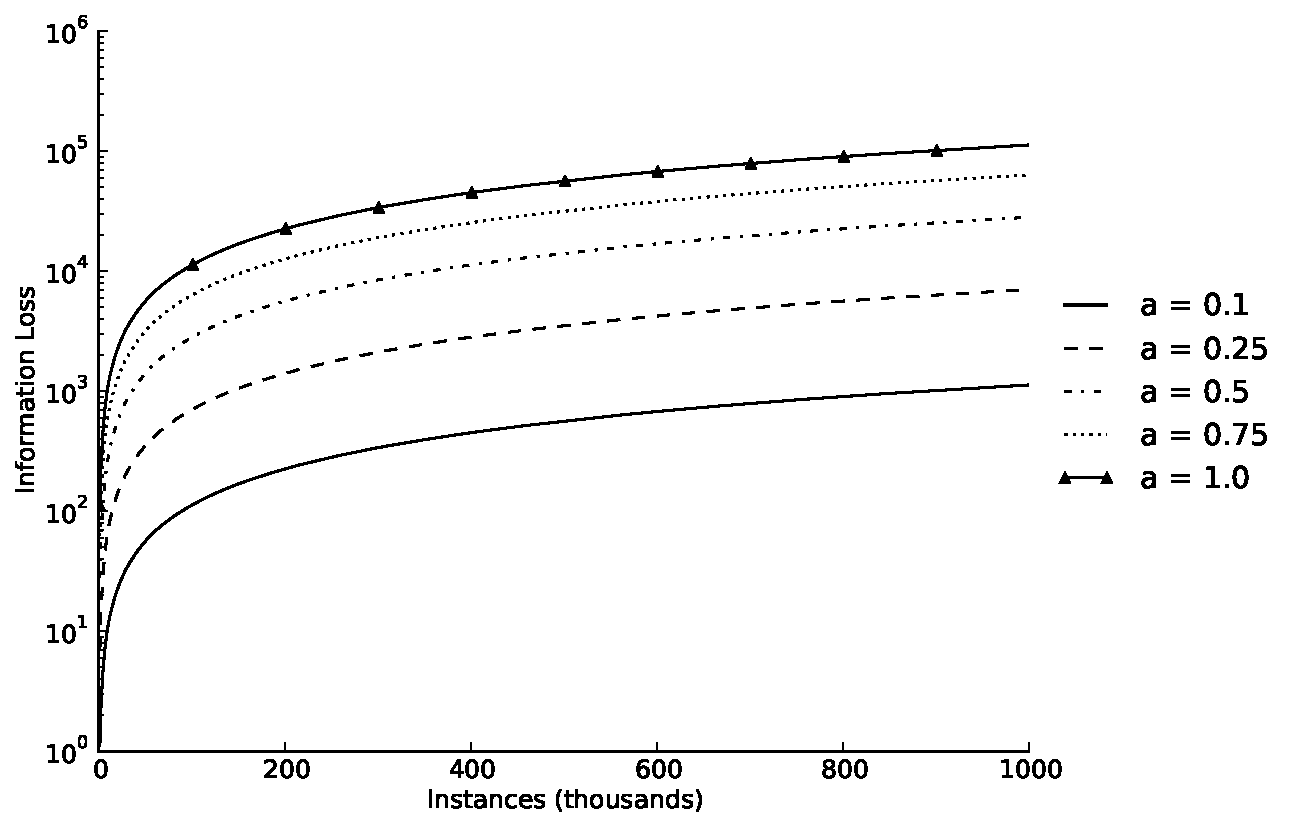
\includegraphics[width=0.9\linewidth]{figures/il-log_na-random.pdf}
	\caption[Noise addition IL evaluation ($c = 0$), logarithmic scale.]{\texttt{NoiseAdditionFilter} IL evaluation using the \texttt{RandomRBFGenerator} with fixed parameter $c = 0$, on a logarithmic scale.}
	\label{fig:results-il-log-na}
\end{figure}

\clearpage

\subsection{Microaggregation}
\label{Benchmarking:Results:MicroAgg}

Tables \ref{table:results-rbf-microaggregation} and \ref{table:results-wave-microaggregation} show the final values for both information loss and disclosure risk for increasing values of the cluster size of the partition step of the microaggregation algorithm (the $k$ parameter) and a fixed historical buffer size of $b = 100$. Additional tables are provided in~\aref{AppendixA} for the rest of the considered buffer sizes. The evolution of disclosure risk against the number of instances processed for the \texttt{MicroaggregationFilter} is shown in~\fref{fig:results-dr-ma} and information loss is shown in~\fref{fig:results-il-log-ma}.

\begin{minipage}[t]{0.5\textwidth}
	\begin{flushleft}
	\begin{table}[H]
		\centering
		\begin{tabular}{@{}rrrr@{}}
			\toprule
			$b$ & $k$ & \multicolumn{1}{c}{DR} & \multicolumn{1}{c}{IL} \\ \midrule
			100  & 3   & 0.232 & 74917.30  \\
			100  & 5   & 0.144 & 89953.68  \\
			100  & 10  & 0.089 & 101193.72 \\
			100  & 15  & 0.069 & 104952.79 \\
			100  & 20  & 0.061 & 106800.51 \\
			100  & 25  & 0.055 & 107937.42 \\
			100  & 50  & 0.041 & 110179.72 \\
			100  & 100 & 0.030 & 111313.78 \\ \bottomrule
		\end{tabular}
		\caption[Microaggregation DR \& IL estimations (\texttt{RandomRBFGenerator}).]{Microaggregation IL \& DR estimations for increasing $k$ (cluster size) and fixed buffer size $b=100$ with the \texttt{RandomRBFGenerator}.}
		\label{table:results-rbf-microaggregation}
	\end{table}
	\end{flushleft}
\end{minipage}
\begin{minipage}[t]{0.5\textwidth}
	\begin{flushright}
	\begin{table}[H]
		\centering
		\begin{tabular}{@{}rrrr@{}}
			\toprule
			$b$ & $k$ & \multicolumn{1}{c}{DR} & \multicolumn{1}{c}{IL} \\ \midrule
			100  & 3   & 0.241 & 3375656.78 \\
			100  & 5   & 0.135 & 4057649.13 \\
			100  & 10  & 0.076 & 4566550.54 \\
			100  & 15  & 0.061 & 4739204.47 \\
			100  & 20  & 0.054 & 4822716.29 \\
			100  & 25  & 0.049 & 4872587.52 \\
			100  & 50  & 0.038 & 4976718.32 \\
			100  & 100 & 0.029 & 5027574.64 \\ \bottomrule
		\end{tabular}
		\caption[Microaggregation DR \& IL estimations (\texttt{WaveformGenerator}).]{Microaggregation IL \& DR estimations for increasing $k$ (cluster size) and fixed buffer size $b=100$ with the \texttt{WaveformGenerator}.}
		\label{table:results-wave-microaggregation}
	\end{table}
	\end{flushright}
\end{minipage}

As shown in the tables above, the \texttt{MicroaggregationFilter} disclosure risk performance is almost the same for both streams (unlike the \texttt{NoiseAdditionFilter}). The total disclosure risk diminishes as the size of the clusters formed increases, which is a direct consequence of the theoretical privacy guarantee that microaggregation offers: because $k$-anonymity is implemented through this algorithmic scheme, the maximum disclosure risk for a given $k$ is $DR \leq 1/k$.

The couple of figures included below show an interesting result of the microaggregation filter. Even though the size of the clusters does not affect too much the amount of noise introduced in the data (see~\fref{fig:results-il-log-ma}), the increase of the of the $k$ parameter offers much better privacy protection than that achieved with lower values. We can anonymize data, obtaining good (low) disclosure risk and not losing too much utility in the process with respect to configurations that yield poorer disclosure risk results.

\begin{figure}[h]
	\centering
	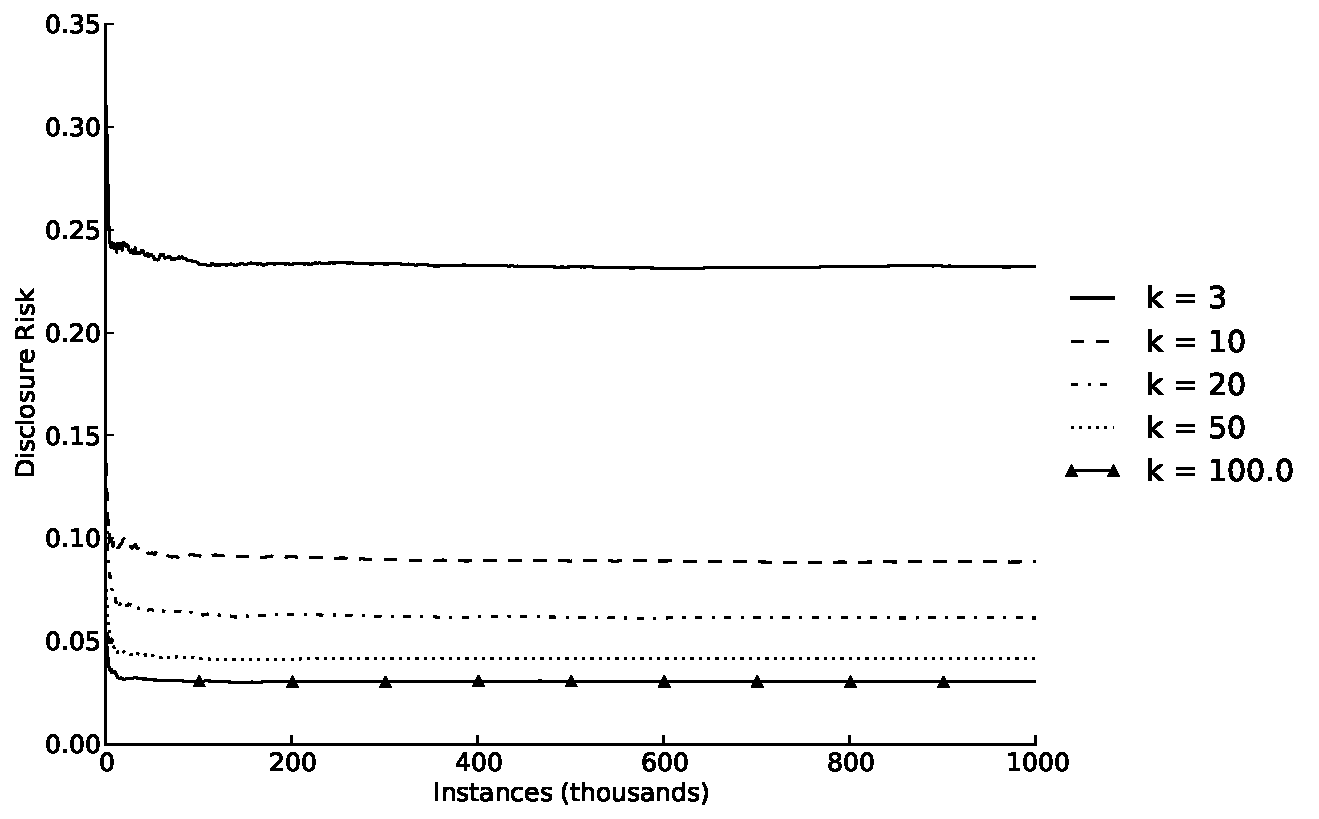
\includegraphics[width=0.9\linewidth]{figures/dr_ma-random.pdf}
	\caption[Microaggregation DR evaluation ($b = 100$).]{\texttt{MicroaggregationFilter} DR evaluation using the \texttt{RandomRBFGenerator} with fixed buffer size $b = 100$, for increasing $k$.}
	\label{fig:results-dr-ma}
\end{figure}

\begin{figure}[h]
	\centering
	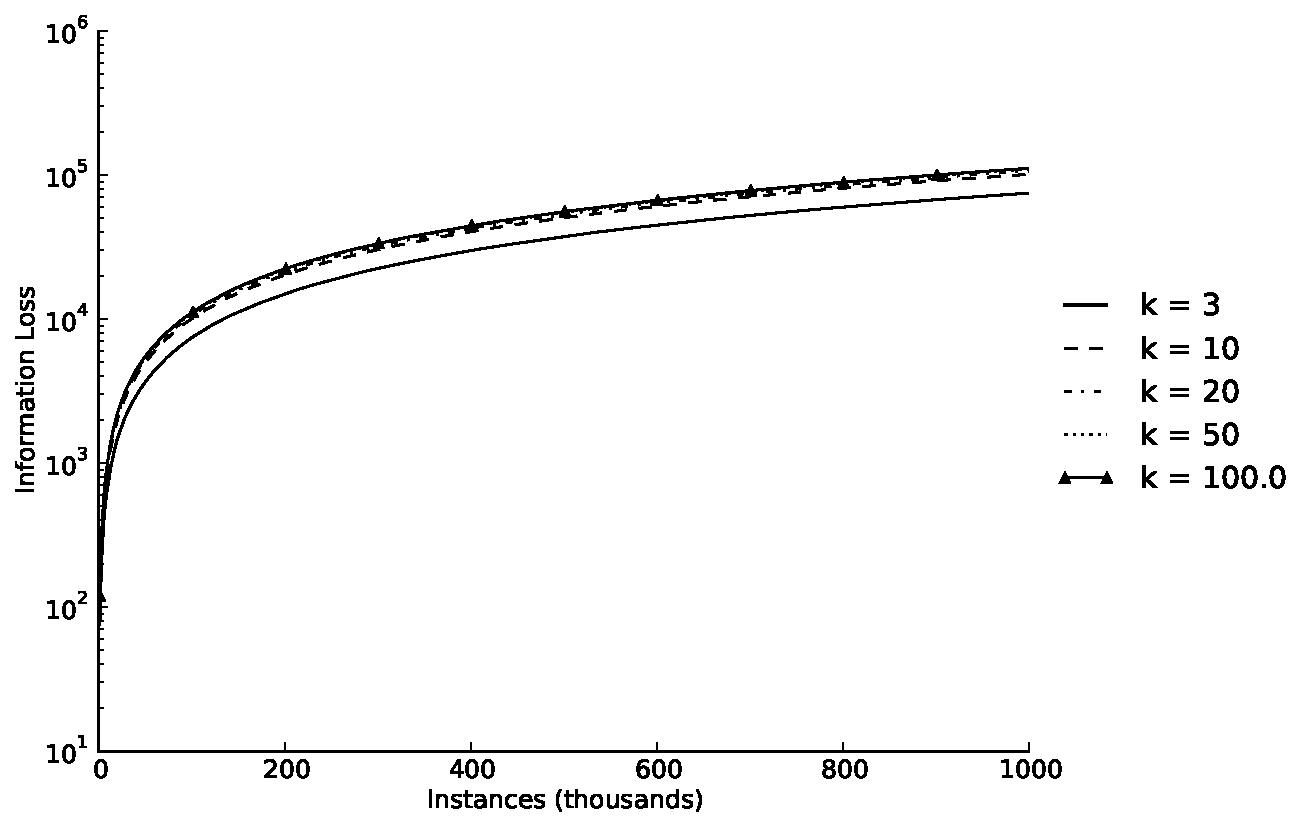
\includegraphics[width=0.9\linewidth]{figures/il-log_ma-random.pdf}
	\caption[Microaggregation IL evaluation ($b = 100$), logarithmic scale.]{\texttt{MicroaggregationFilter} IL evaluation using the \texttt{RandomRBFGenerator} with fixed buffer size $b = 100$, for increasing $k$, on a logarithmic scale.}
	\label{fig:results-il-log-ma}
\end{figure}

\clearpage

\subsection{Rank swapping}
\label{Benchmarking:Results:RankSwap}

A comparison of the performance of the \texttt{RankSwappingFilter} on the streams produced by the \texttt{RandomRBFGenerator} and \texttt{WaveformGenerator} can be seen in~\tref{table:results-rbf-rankswap} and~\tref{table:results-wave-rankswap}. The remaining tables of results can be consulted in the~\aref{AppendixA}. \fref{fig:results-dr-rs} shows the disclosure risk estimation against the number of instances processed, for increasing values of the $p$ parameter and two buffer sizes ($b = 100$ and $b=500$). The information loss estimate of the corresponding parameterizations is shown in~\fref{fig:results-il-log-rs}.

\begin{minipage}[t]{0.5\textwidth}
	\begin{flushleft}
	\begin{table}[H]
		\centering
		\begin{tabular}{@{}rrrr@{}}
			\toprule
			$b$ & $p$ & \multicolumn{1}{c}{DR} & \multicolumn{1}{c}{IL} \\ \midrule
			100  & 10 & 0.838 & 19136.62  \\
			100  & 25 & 0.469 & 57753.05  \\
			100  & 50 & 0.070 & 136791.17 \\
			100  & 75 & 0.036 & 178200.11 \\
			100  & 80 & 0.037 & 178685.81 \\ \bottomrule
		\end{tabular}
		\caption[Rank swapping DR \& IL estimations (\texttt{RandomRBFGenerator}).]{Rank swapping IL \& DR estimations for increasing $p$ (maximum swap range) and fixed buffer size $b=100$ with the \texttt{RandomRBFGenerator}.}
		\label{table:results-rbf-rankswap}
	\end{table}
	\end{flushleft}
\end{minipage}
\begin{minipage}[t]{0.5\textwidth}
	\begin{flushright}
	\begin{table}[H]
		\centering
		\begin{tabular}{@{}rrrr@{}}
			\toprule
			$b$ & $p$ & \multicolumn{1}{c}{DR} & \multicolumn{1}{c}{IL} \\ \midrule
			100  & 10 & 0.997 & 705196.07  \\
			100  & 25 & 0.776 & 2464673.56 \\
			100  & 50 & 0.112 & 6195304.18 \\
			100  & 75 & 0.046 & 8088473.27 \\
			100  & 80 & 0.045 & 8097619.70 \\ \bottomrule
		\end{tabular}
		\caption[Rank swapping DR \& IL estimations (\texttt{WaveformGenerator}).]{Rank swapping IL \& DR estimations for increasing $p$ (maximum swap range) and fixed buffer size $b=100$ with the \texttt{WaveformGenerator}.}
		\label{table:results-wave-rankswap}
	\end{table}
	\end{flushright}
\end{minipage}

As we see in both~\tref{table:results-rbf-rankswap} and~\tref{table:results-wave-rankswap}, the maximum swap range, defined as the percentage $p$ of the size of the buffer, is indeed a key factor to achieve good results, concerning the disclosure risk of the anonymized data. Both tables show that, for swap ranges shorter than half the size of the window, the risk or fe-identification is too high.

The remaining parameter of this filter, the size of the buffer, is also, in this case, an important factor to leverage when using the \texttt{RankSwappingFilter}. For bigger buffer sizes, the information loss incurred decreases, but the disclosure risk grows too much. The cause behind this increase in the revelation risk could be the usage of synthetical data: for bigger buffer sizes, because generated attribute values are sensibly close to each other, the difference between the swapped values is smaller, thus generating lower noise and exposing more information to an attacker.

\begin{figure}[h]
	\centering
	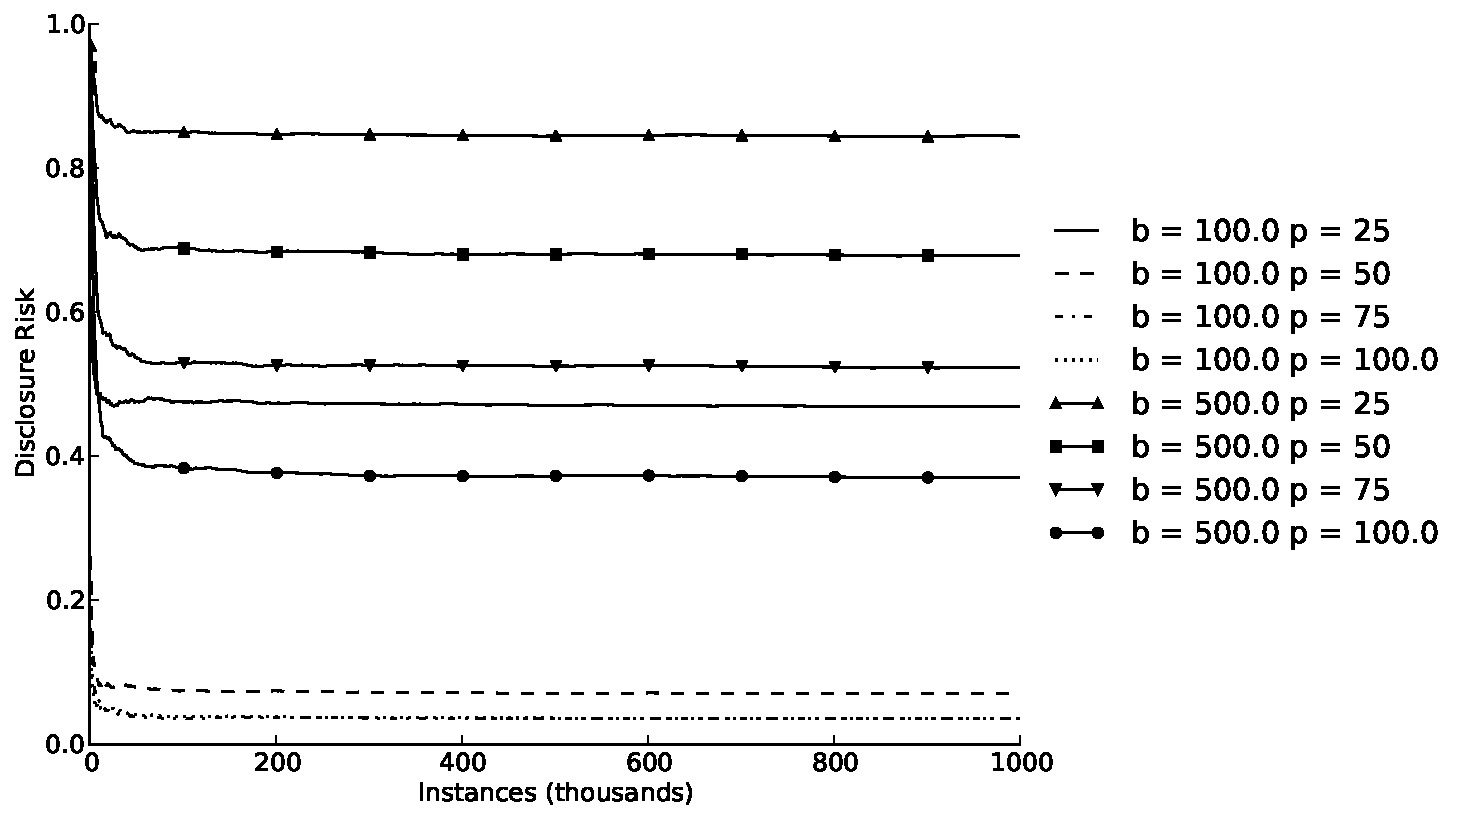
\includegraphics[width=1.0\linewidth]{figures/dr_rs-random.pdf}
	\caption[Rank swapping DR evaluation ($b = \{100,500\}$).]{\texttt{RankSwappingFilter} DR evaluation using the \texttt{RandomRBFGenerator} with buffer sizes $b = 100$ and $b = 500$, for increasing $p$.}
	\label{fig:results-dr-rs}
\end{figure}

\begin{figure}[h]
	\centering
	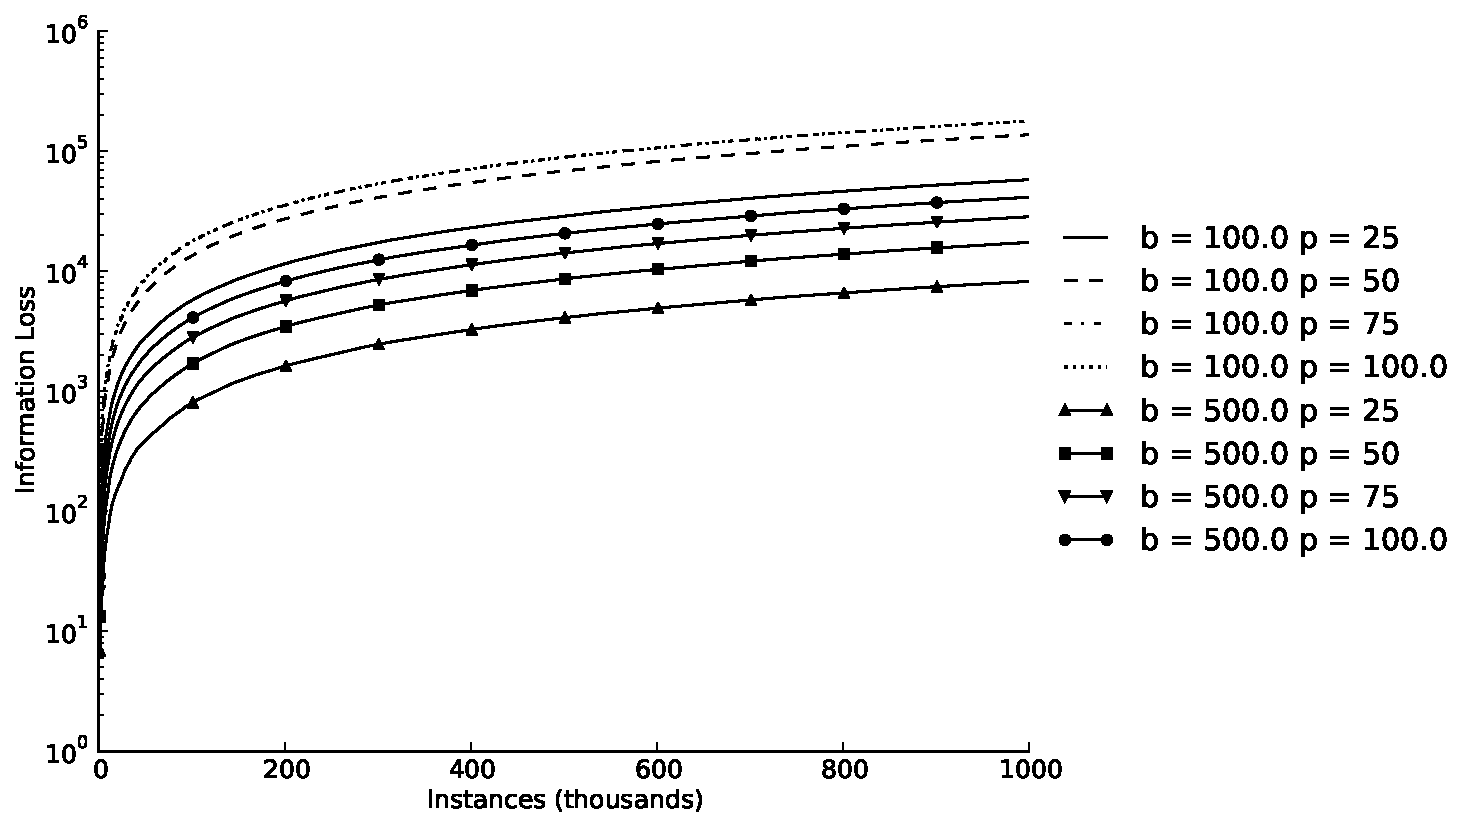
\includegraphics[width=1.0\linewidth]{figures/il-log_rs-random.pdf}
	\caption[Rank swapping IL evaluation ($b = \{100,500\}$), logarithmic scale.]{\texttt{RankSwappingFilter} IL evaluation using the \texttt{RandomRBFGenerator} with buffer sizes $b = 100$ and $b = 500$, for increasing $p$, on a logarithmic scale.}
	\label{fig:results-il-log-rs}
\end{figure}

\clearpage

\subsection{$\varepsilon$-Differential private microaggregation}
\label{Benchmarking:Results:DiffPriv}

An aggregate of five ``subtables'' is shown in~\tref{table:results-random-diff-priv}: the disclosure risk and information loss results are assessed for increasing values of cluster size $k$, increasing differential privacy scale factors, controlled by the $\varepsilon$ parameter, and fixed historical buffer size $b = 250$. The complete set of results tables is located in~\aref{AppendixA}.

\begin{figure}[h]
	\centering
	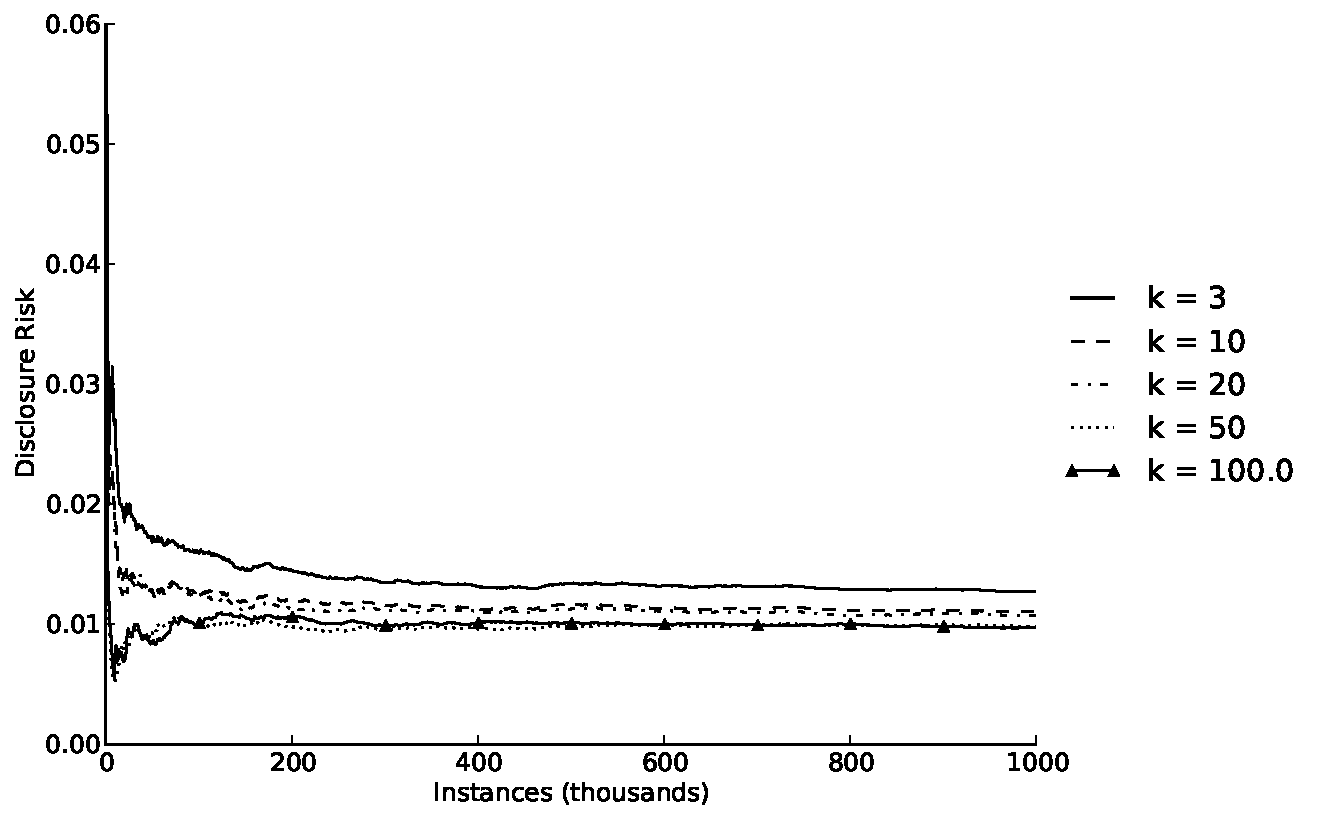
\includegraphics[width=0.9\linewidth]{figures/dr_dp-e1-random.pdf}
	\caption[Differential privacy DR evaluation ($b = 100,~\varepsilon = 1$).]{\texttt{DifferentialPrivacyFilter} DR evaluation using the \texttt{RandomRBFGenerator} with fixed buffer size $b = 100$ and fixed differential privacy scale parameter $\varepsilon = 1$, for increasing $k$.}
	\label{fig:results-dr-dp-e1}
\end{figure}

The \texttt{DifferentialPrivacyFilter} performs really well in terms of disclosure risk, for any of the parameters combinations displayed. However, for small values of $\varepsilon$, the amount of noise added to data is really high. Confirming the hipothesis presented in~\sref{Implementation:DifferentialPrivacy:Design}, increasing the size of the clusters $k$ achieves a reduction in the sensitivity of the release function of the data, thus reducing the Laplacian noise introduced, thus reducing information loss. This effect can be seen for values of $\varepsilon$ up to $10$, but is not visible for $\varepsilon = 100$, because, for such a high $\varepsilon$, the majority of the added noise is indeed caused by the microaggregation function, not by the Laplace mechanism. This effect can also be assessed in~\fref{fig:results-il-dp-e1}, where the value of $\varepsilon$ is fixed and $k$ increases, effectively reducing information loss.

\begin{table}[H]
	\centering
	\begin{tabular}{@{}cc@{}}
		\begin{tabular}{@{}rrrrr@{}}
			\toprule
			$b$ & $\varepsilon$ & $k$ & \multicolumn{1}{c}{DR} & \multicolumn{1}{c}{IL} \\ \midrule
			250 & 0.01 & 3   & 0.004 & 3.298E+11 \\
			250 & 0.01 & 5   & 0.004 & 2.483E+11 \\
			250 & 0.01 & 10  & 0.004 & 2.033E+11 \\
			250 & 0.01 & 15  & 0.005 & 1.885E+11 \\
			250 & 0.01 & 20  & 0.004 & 1.880E+11 \\
			250 & 0.01 & 25  & 0.004 & 1.881E+11 \\
			250 & 0.01 & 50  & 0.005 & 1.502E+11 \\
			250 & 0.01 & 100 & 0.005 & 1.050E+11 \\ \bottomrule
		\end{tabular}
		&
		\begin{tabular}{@{}rrrrr@{}}
			\toprule
			$b$ & $\varepsilon$ & $k$ & \multicolumn{1}{c}{DR} & \multicolumn{1}{c}{IL} \\ \midrule
			250 & 0.1 & 3   & 0.005 & 3.298E+09 \\
			250 & 0.1 & 5   & 0.005 & 2.483E+09 \\
			250 & 0.1 & 10  & 0.004 & 2.033E+09 \\
			250 & 0.1 & 15  & 0.005 & 1.885E+09 \\
			250 & 0.1 & 20  & 0.005 & 1.880E+09 \\
			250 & 0.1 & 25  & 0.004 & 1.881E+09 \\
			250 & 0.1 & 50  & 0.005 & 1.502E+09 \\
			250 & 0.1 & 100 & 0.005 & 1.050E+09 \\ \bottomrule
		\end{tabular}
		\\ & \\
		\begin{tabular}{@{}rrrrr@{}}
			\toprule
			$b$ & $\varepsilon$ & $k$ & \multicolumn{1}{c}{DR} & \multicolumn{1}{c}{IL} \\ \midrule
			250 & 1.0 & 3   & 0.006 & 3.305E+07 \\
			250 & 1.0 & 5   & 0.005 & 2.492E+07 \\
			250 & 1.0 & 10  & 0.005 & 2.043E+07 \\
			250 & 1.0 & 15  & 0.005 & 1.896E+07 \\
			250 & 1.0 & 20  & 0.005 & 1.890E+07 \\
			250 & 1.0 & 25  & 0.005 & 1.892E+07 \\
			250 & 1.0 & 50  & 0.005 & 1.513E+07 \\
			250 & 1.0 & 100 & 0.005 & 1.062E+07 \\ \bottomrule
		\end{tabular}
		&
		\begin{tabular}{@{}rrrrr@{}}
			\toprule
			$b$ & $\varepsilon$ & $k$ & \multicolumn{1}{c}{DR} & \multicolumn{1}{c}{IL} \\ \midrule
			250 & 10 & 3   & 0.032 & 3.985E+05 \\
			250 & 10 & 5   & 0.019 & 3.345E+05 \\
			250 & 10 & 10  & 0.012 & 3.021E+05 \\
			250 & 10 & 15  & 0.011 & 2.917E+05 \\
			250 & 10 & 20  & 0.010 & 2.934E+05 \\
			250 & 10 & 25  & 0.009 & 2.950E+05 \\
			250 & 10 & 50  & 0.006 & 2.600E+05 \\
			250 & 10 & 100 & 0.005 & 2.164E+05 \\ \bottomrule
		\end{tabular}
		\\ & \\
		\multicolumn{2}{c}{
			\begin{tabular}{@{}rrrrr@{}}
				\toprule
				$b$ & $\varepsilon$ & $k$ & \multicolumn{1}{c}{DR} & \multicolumn{1}{c}{IL} \\ \midrule
				250 & 100 &  3   & 0.155 & 7.152E+04 \\
				250 & 100 &  5   & 0.079 & 8.824E+04 \\
				250 & 100 &  10  & 0.041 & 1.004E+05 \\
				250 & 100 &  15  & 0.027 & 1.047E+05 \\
				250 & 100 &  20  & 0.022 & 1.069E+05 \\
				250 & 100 &  25  & 0.019 & 1.083E+05 \\
				250 & 100 &  50  & 0.010 & 1.110E+05 \\
				250 & 100 &  100 & 0.006 & 1.122E+05 \\ \bottomrule
			\end{tabular}
		}
	\end{tabular}
	\caption[Differential privacy DR \& IL estimations.]{Differential privacy DR \& IL estimations for increasing $\varepsilon$ and $k$ values and fixed buffer size ($b = 250$). Results from the execution with the \texttt{RandomRBFGenerator}.}
	\label{table:results-random-diff-priv}
\end{table}

\begin{figure}[h]
	\centering
	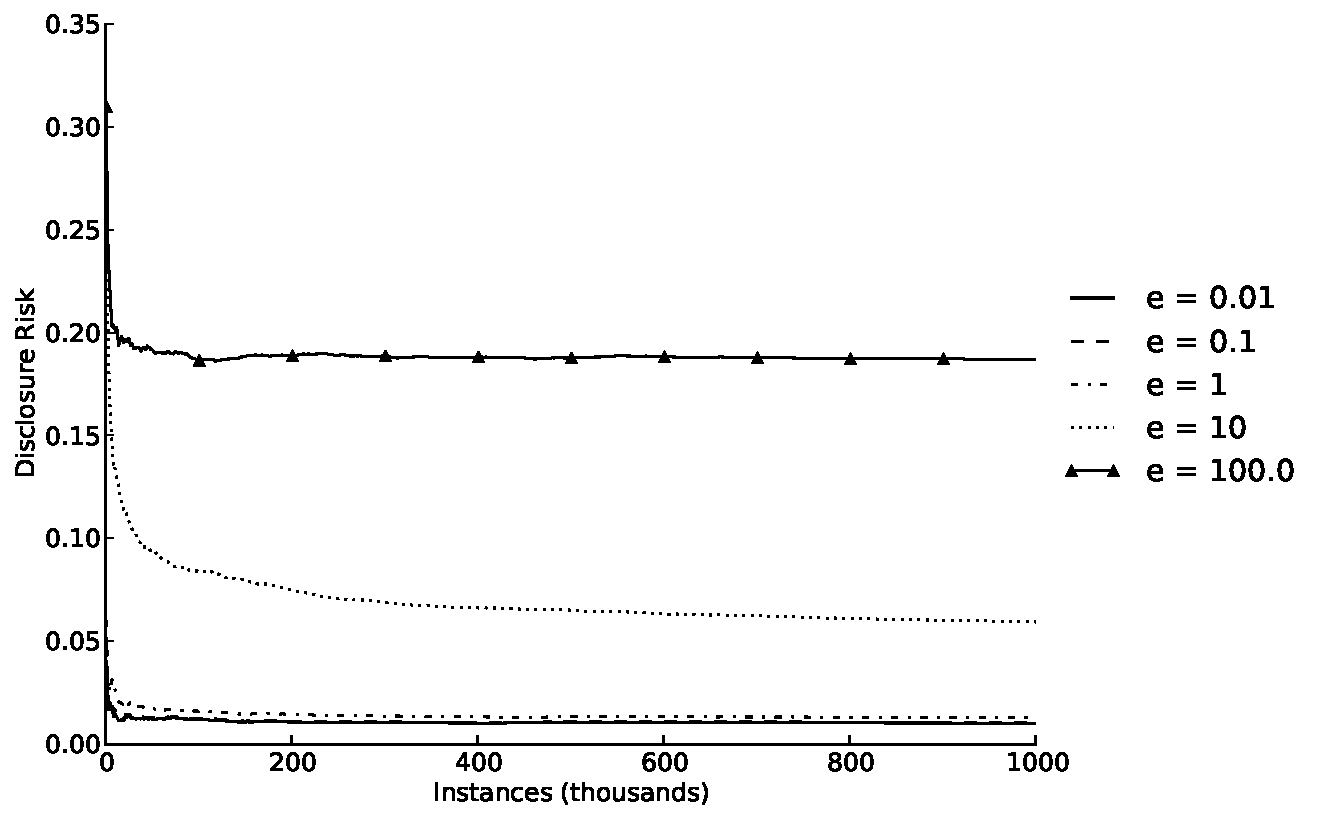
\includegraphics[width=0.9\linewidth]{figures/dr_dp-k3-random.pdf}
	\caption[Differential privacy DR evaluation ($b = 100,~k = 3$).]{\texttt{DifferentialPrivacyFilter} DR evaluation using the \texttt{RandomRBFGenerator} with fixed buffer size $b = 100$ and fixed cluster size $k = 3$, for increasing $\varepsilon$ differential privacy scale factor.}
	\label{fig:results-dr-dp-k3}
\end{figure}

\begin{figure}[h]
	\centering
	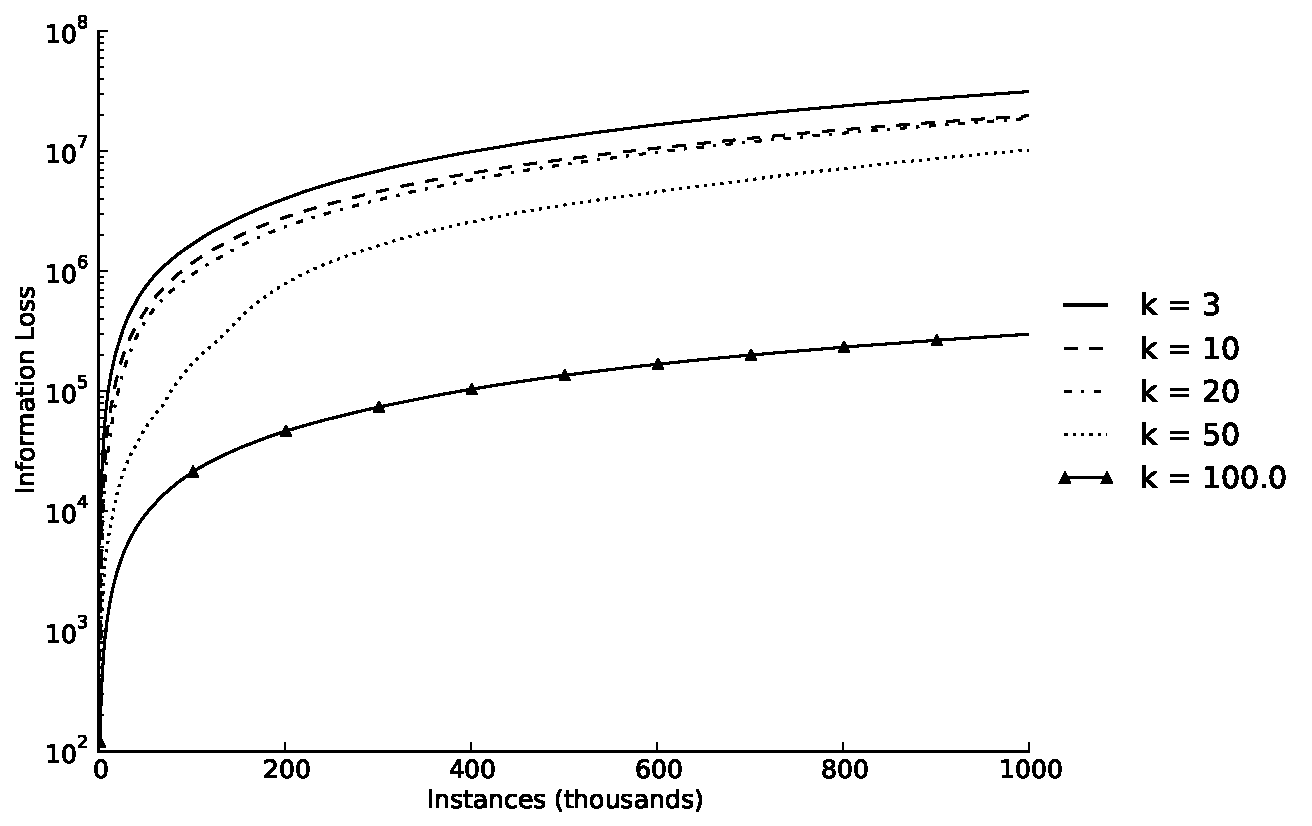
\includegraphics[width=0.9\linewidth]{figures/il-log_dp-e1-random.pdf}
	\caption[Differential privacy IL evaluation ($b = 100,~\varepsilon = 1$).]{\texttt{DifferentialPrivacyFilter} IL evaluation using the \texttt{RandomRBFGenerator} with fixed buffer size $b = 100$ and fixed differential privacy scale parameter $\varepsilon = 1$, for increasing $k$, on a logarithmic scale.}
	\label{fig:results-il-dp-e1}
\end{figure}

\begin{figure}[h]
	\centering
	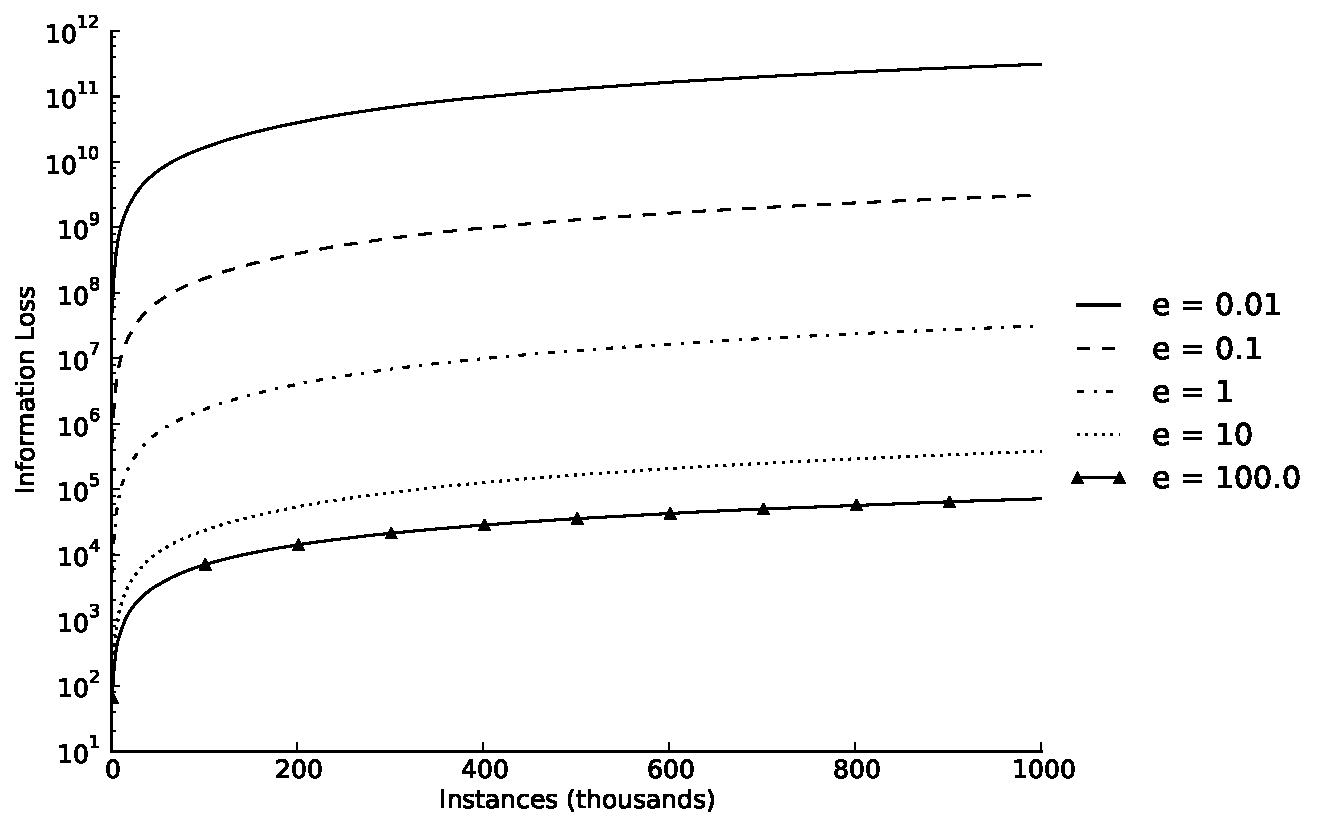
\includegraphics[width=0.9\linewidth]{figures/il-log_dp-k3-random.pdf}
	\caption[Differential privacy IL evaluation ($b = 100,~k = 3$).]{\texttt{DifferentialPrivacyFilter} IL evaluation using the \texttt{RandomRBFGenerator} with fixed buffer size $b = 100$ and fixed cluster size $k = 3$, for increasing $\varepsilon$ differential privacy scale factor, on a logarithmic scale.}
	\label{fig:results-il-dp-k3}
\end{figure}
